\appendix{Представление графического материала}

Графический материал, выполненный на отдельных листах,
изображен на рисунках А.1--А.\arabic{числоПлакатов}.
\setcounter{числоПлакатов}{9}

\renewcommand{\thefigure}{А.\arabic{figure}} % шаблон номера для плакатов

\begin{landscape}
	
\begin{плакат}
	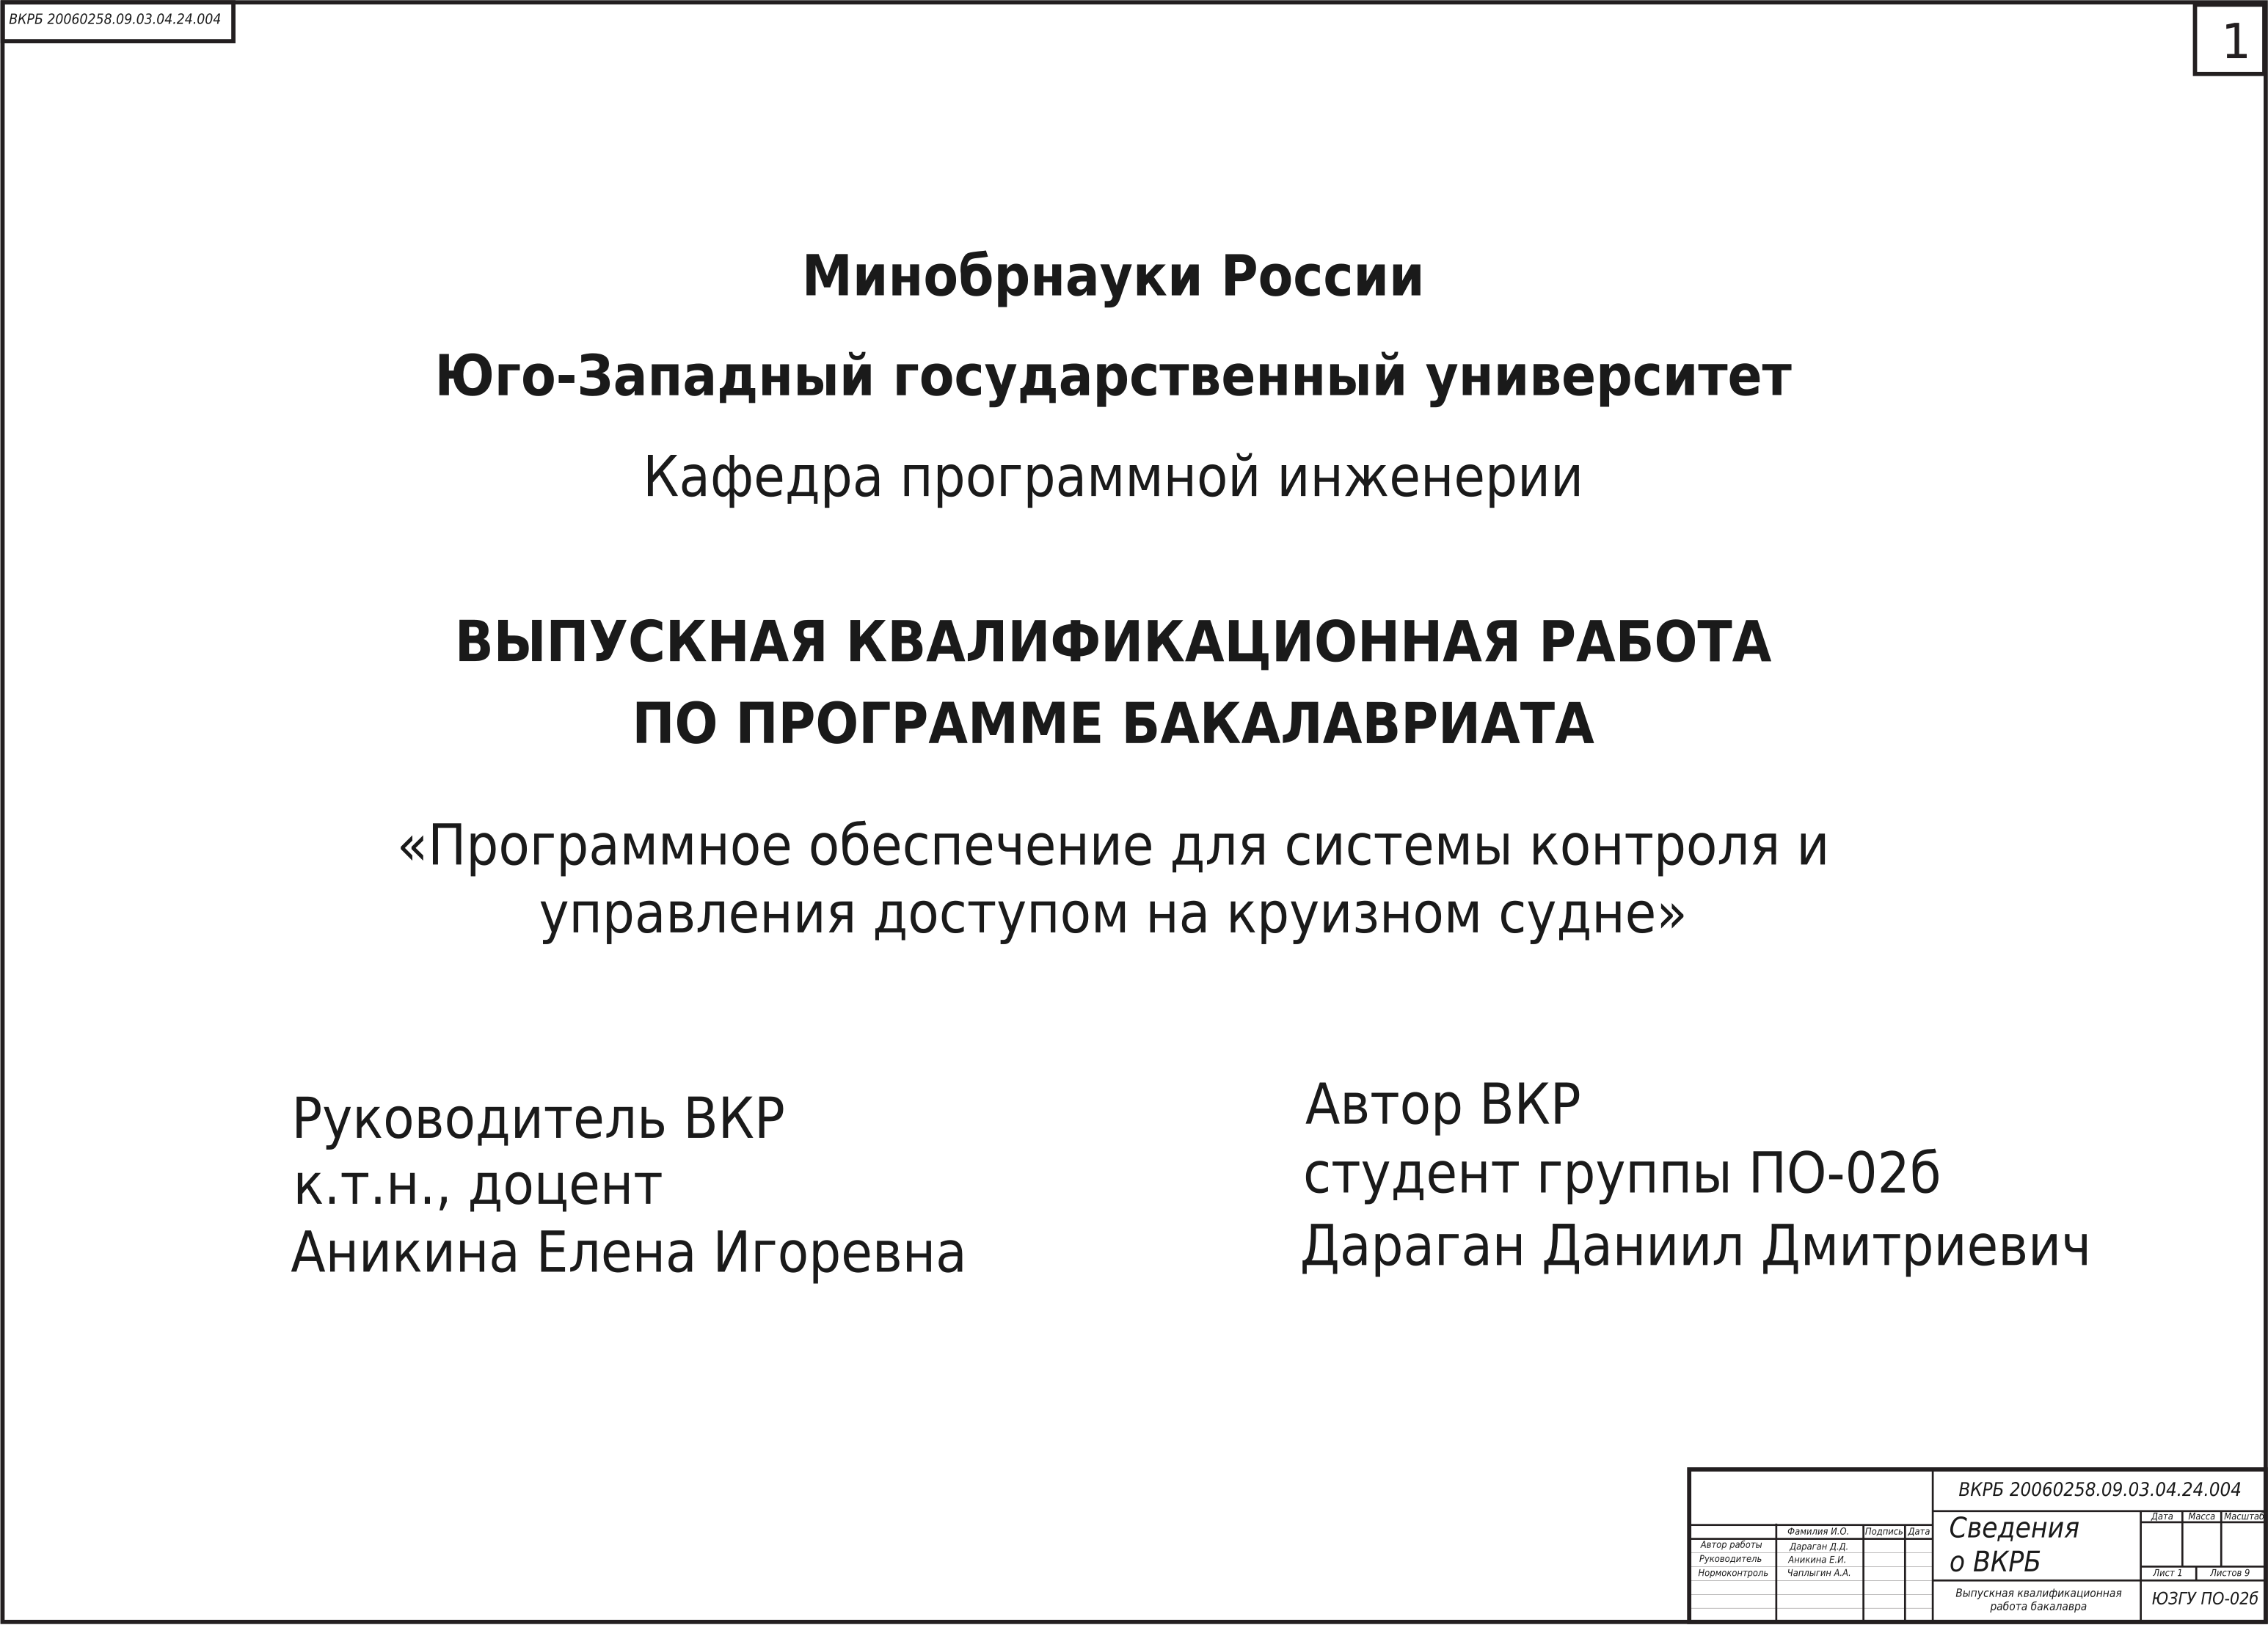
\includegraphics[width=0.82\linewidth]{images/плакат1.png}
	\заголовок{Сведения о ВКРБ}
	\label{fig:1}
\end{плакат}

\begin{плакат}
	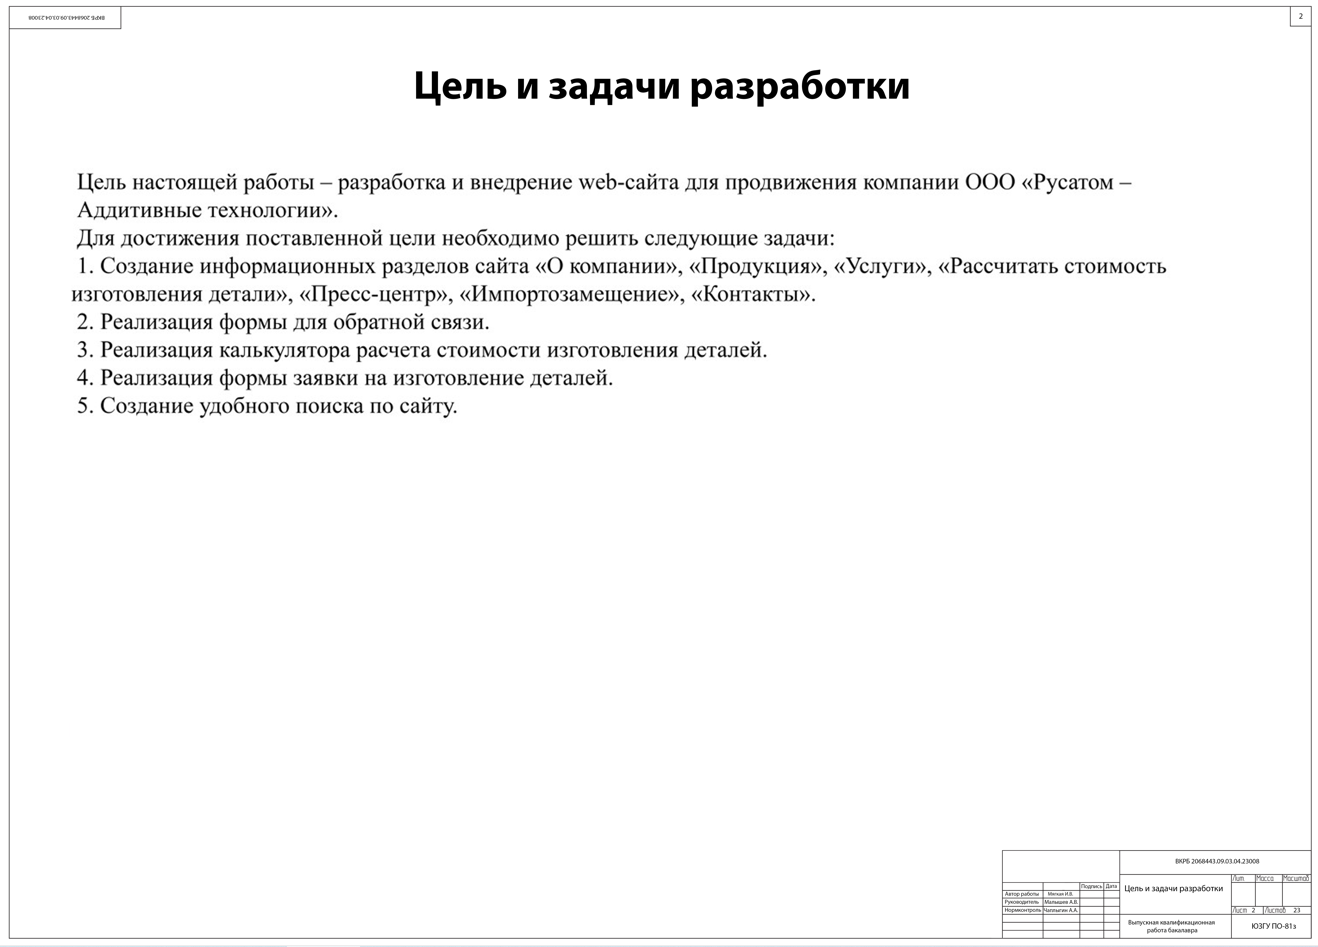
\includegraphics[width=0.82\linewidth]{images/плакат2.png}
	\заголовок{Цель и задачи разработки}
	\label{fig:2}
\end{плакат}

\begin{плакат}
	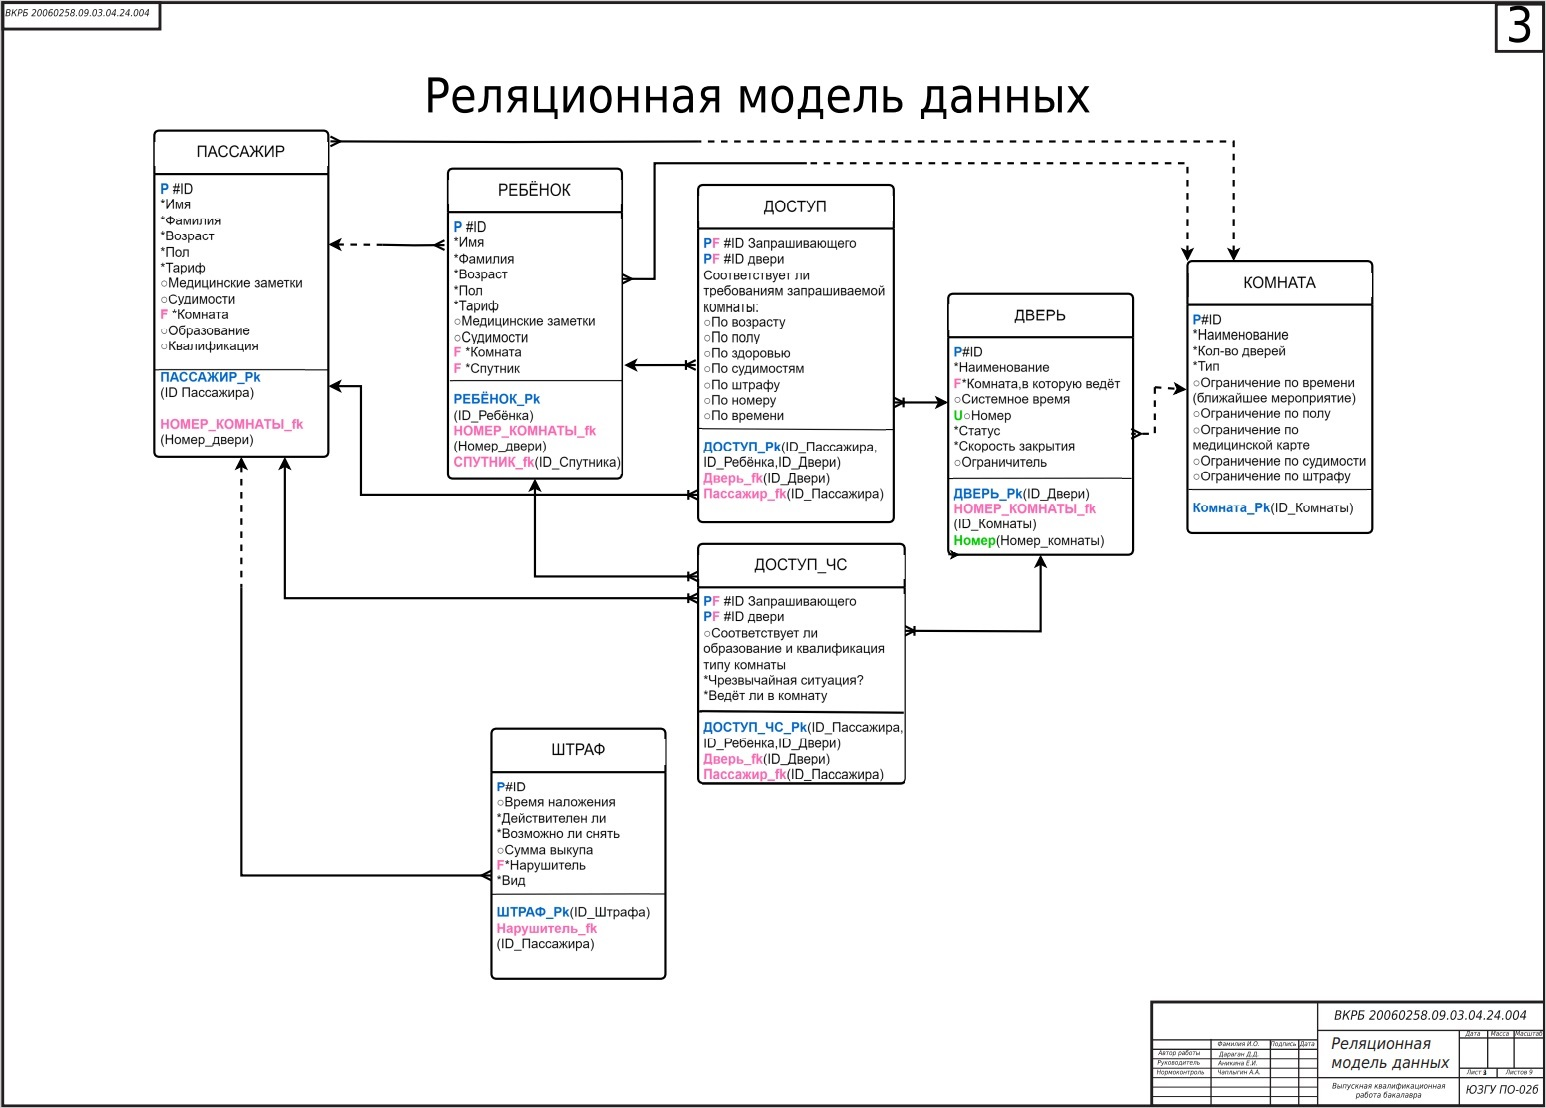
\includegraphics[width=0.82\linewidth]{images/плакат3.png}
	\заголовок{Реляционная модель данных}
	\label{fig:3}
\end{плакат}

\begin{плакат}
	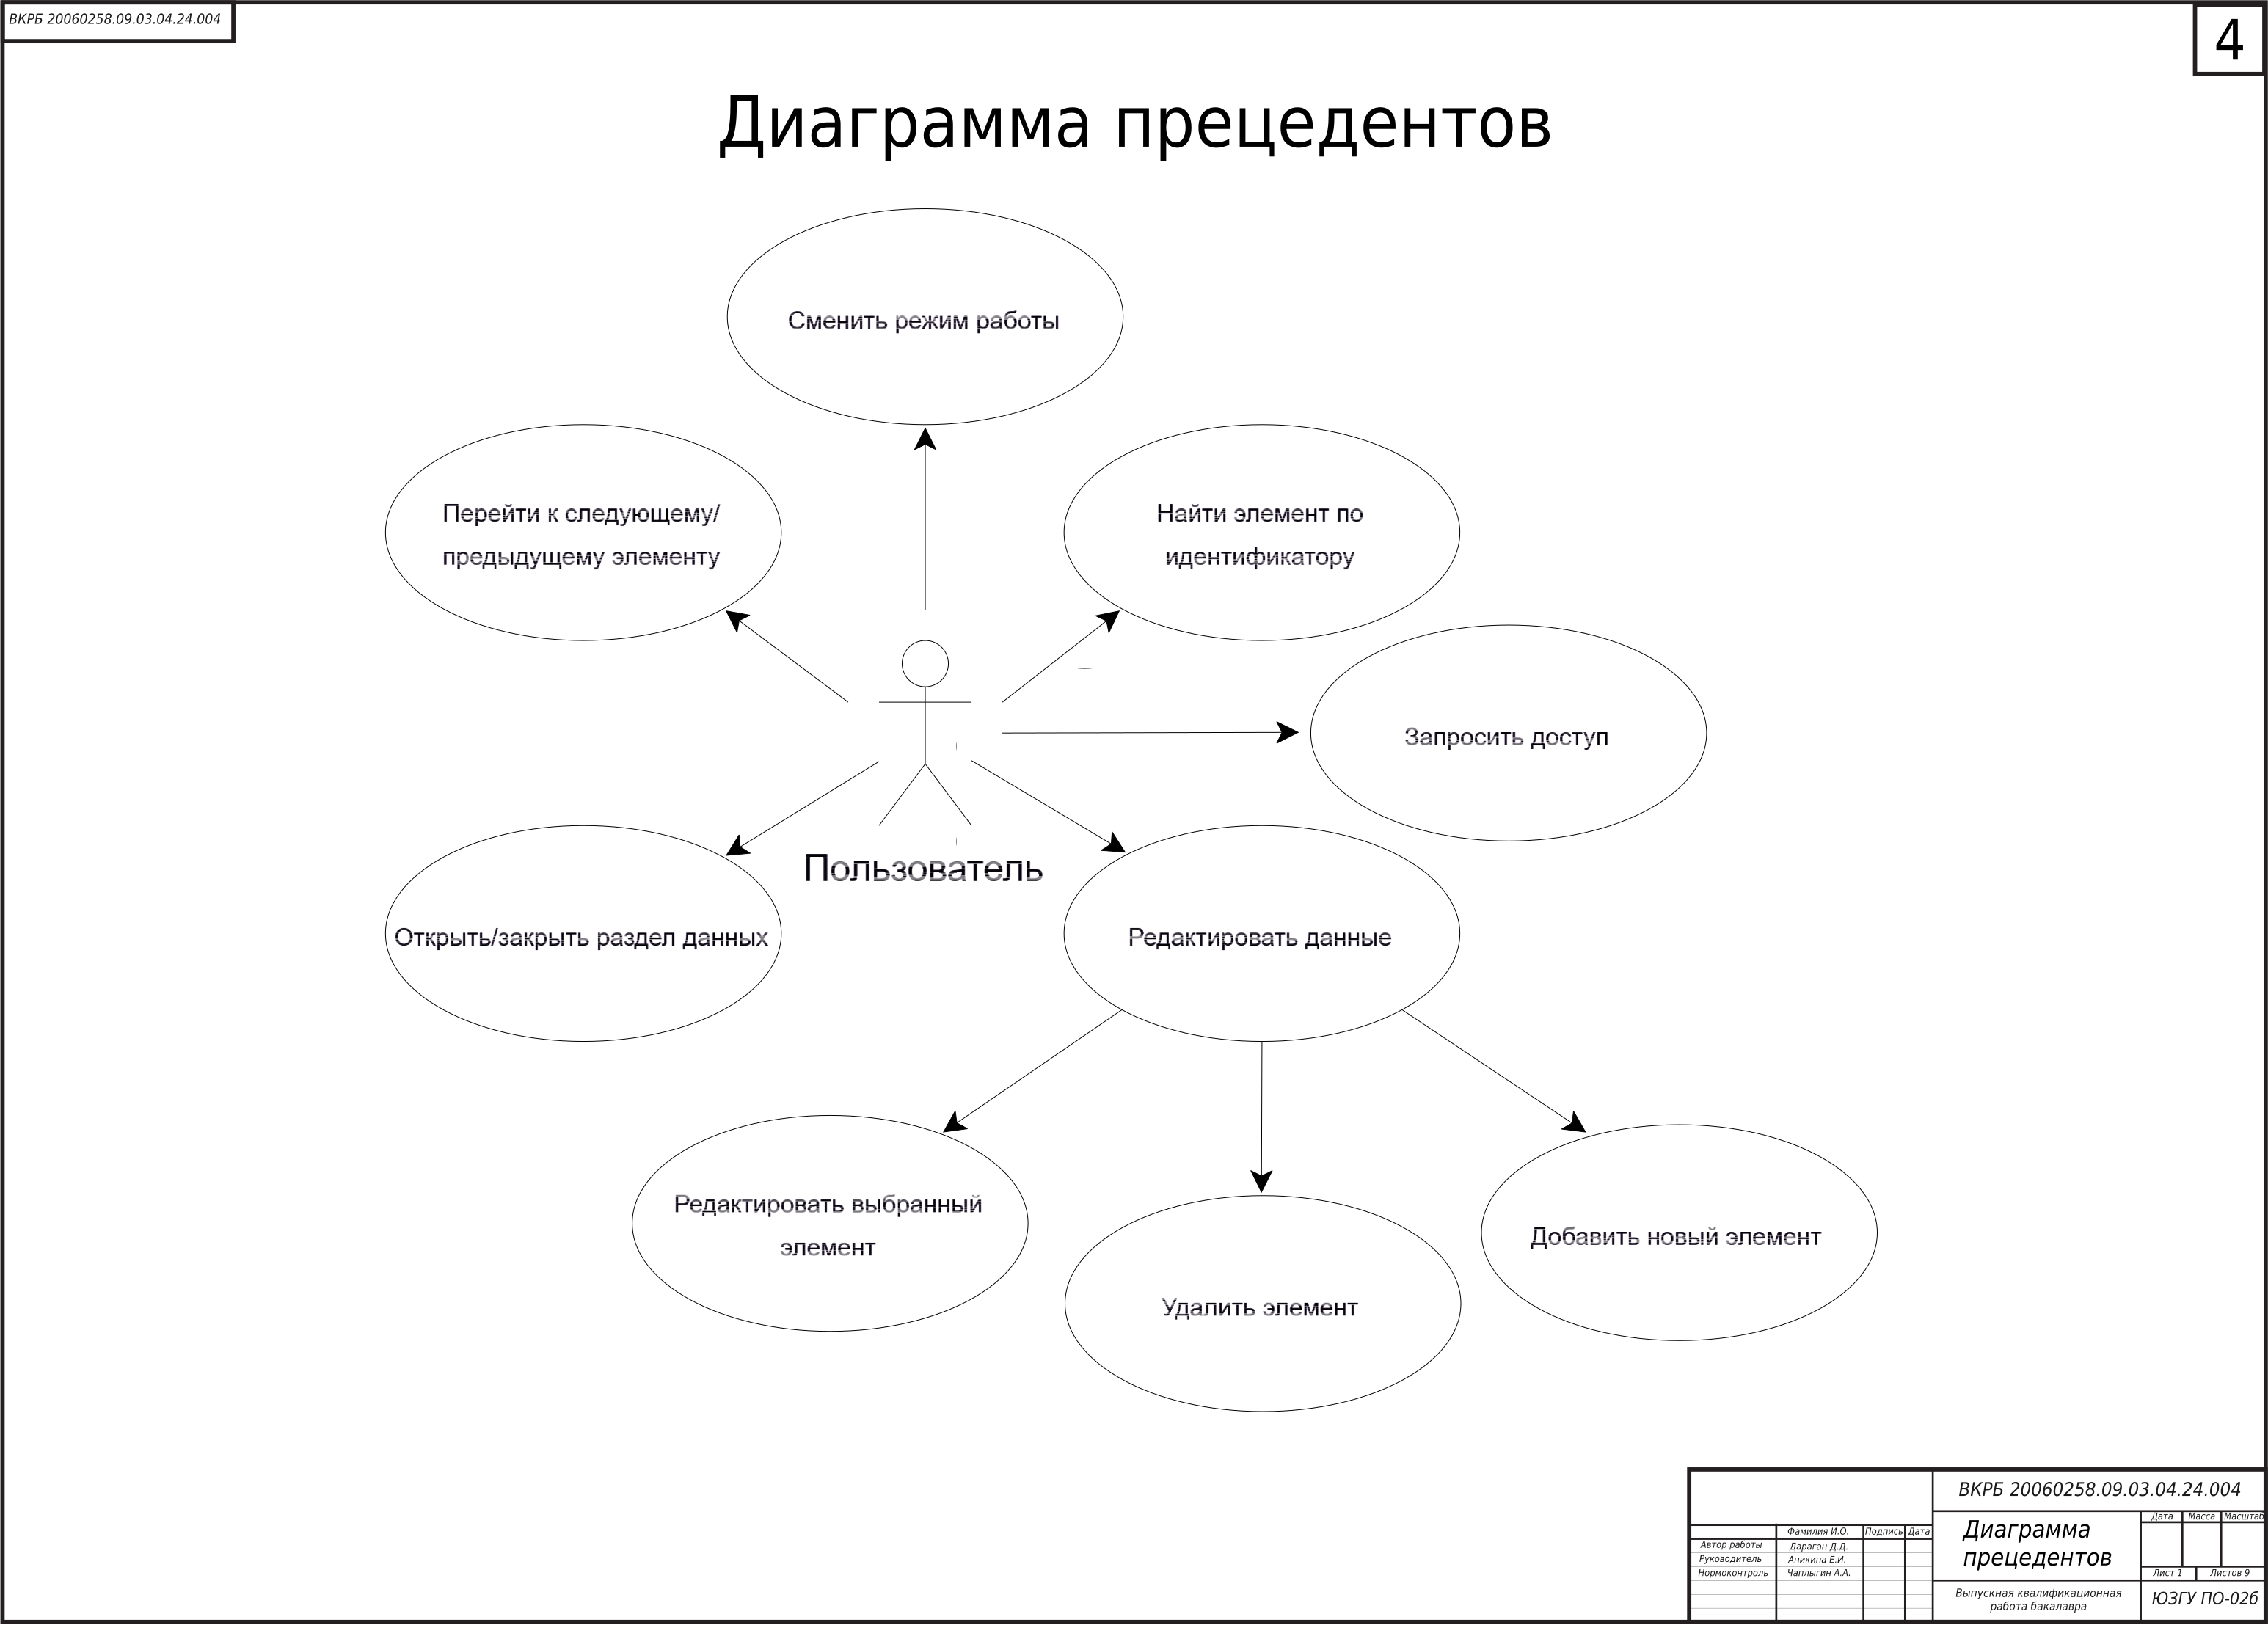
\includegraphics[width=0.82\linewidth]{images/плакат4.png}
	\заголовок{Диаграмма прецедентов}
	\label{fig:4}
\end{плакат}

\begin{плакат}
	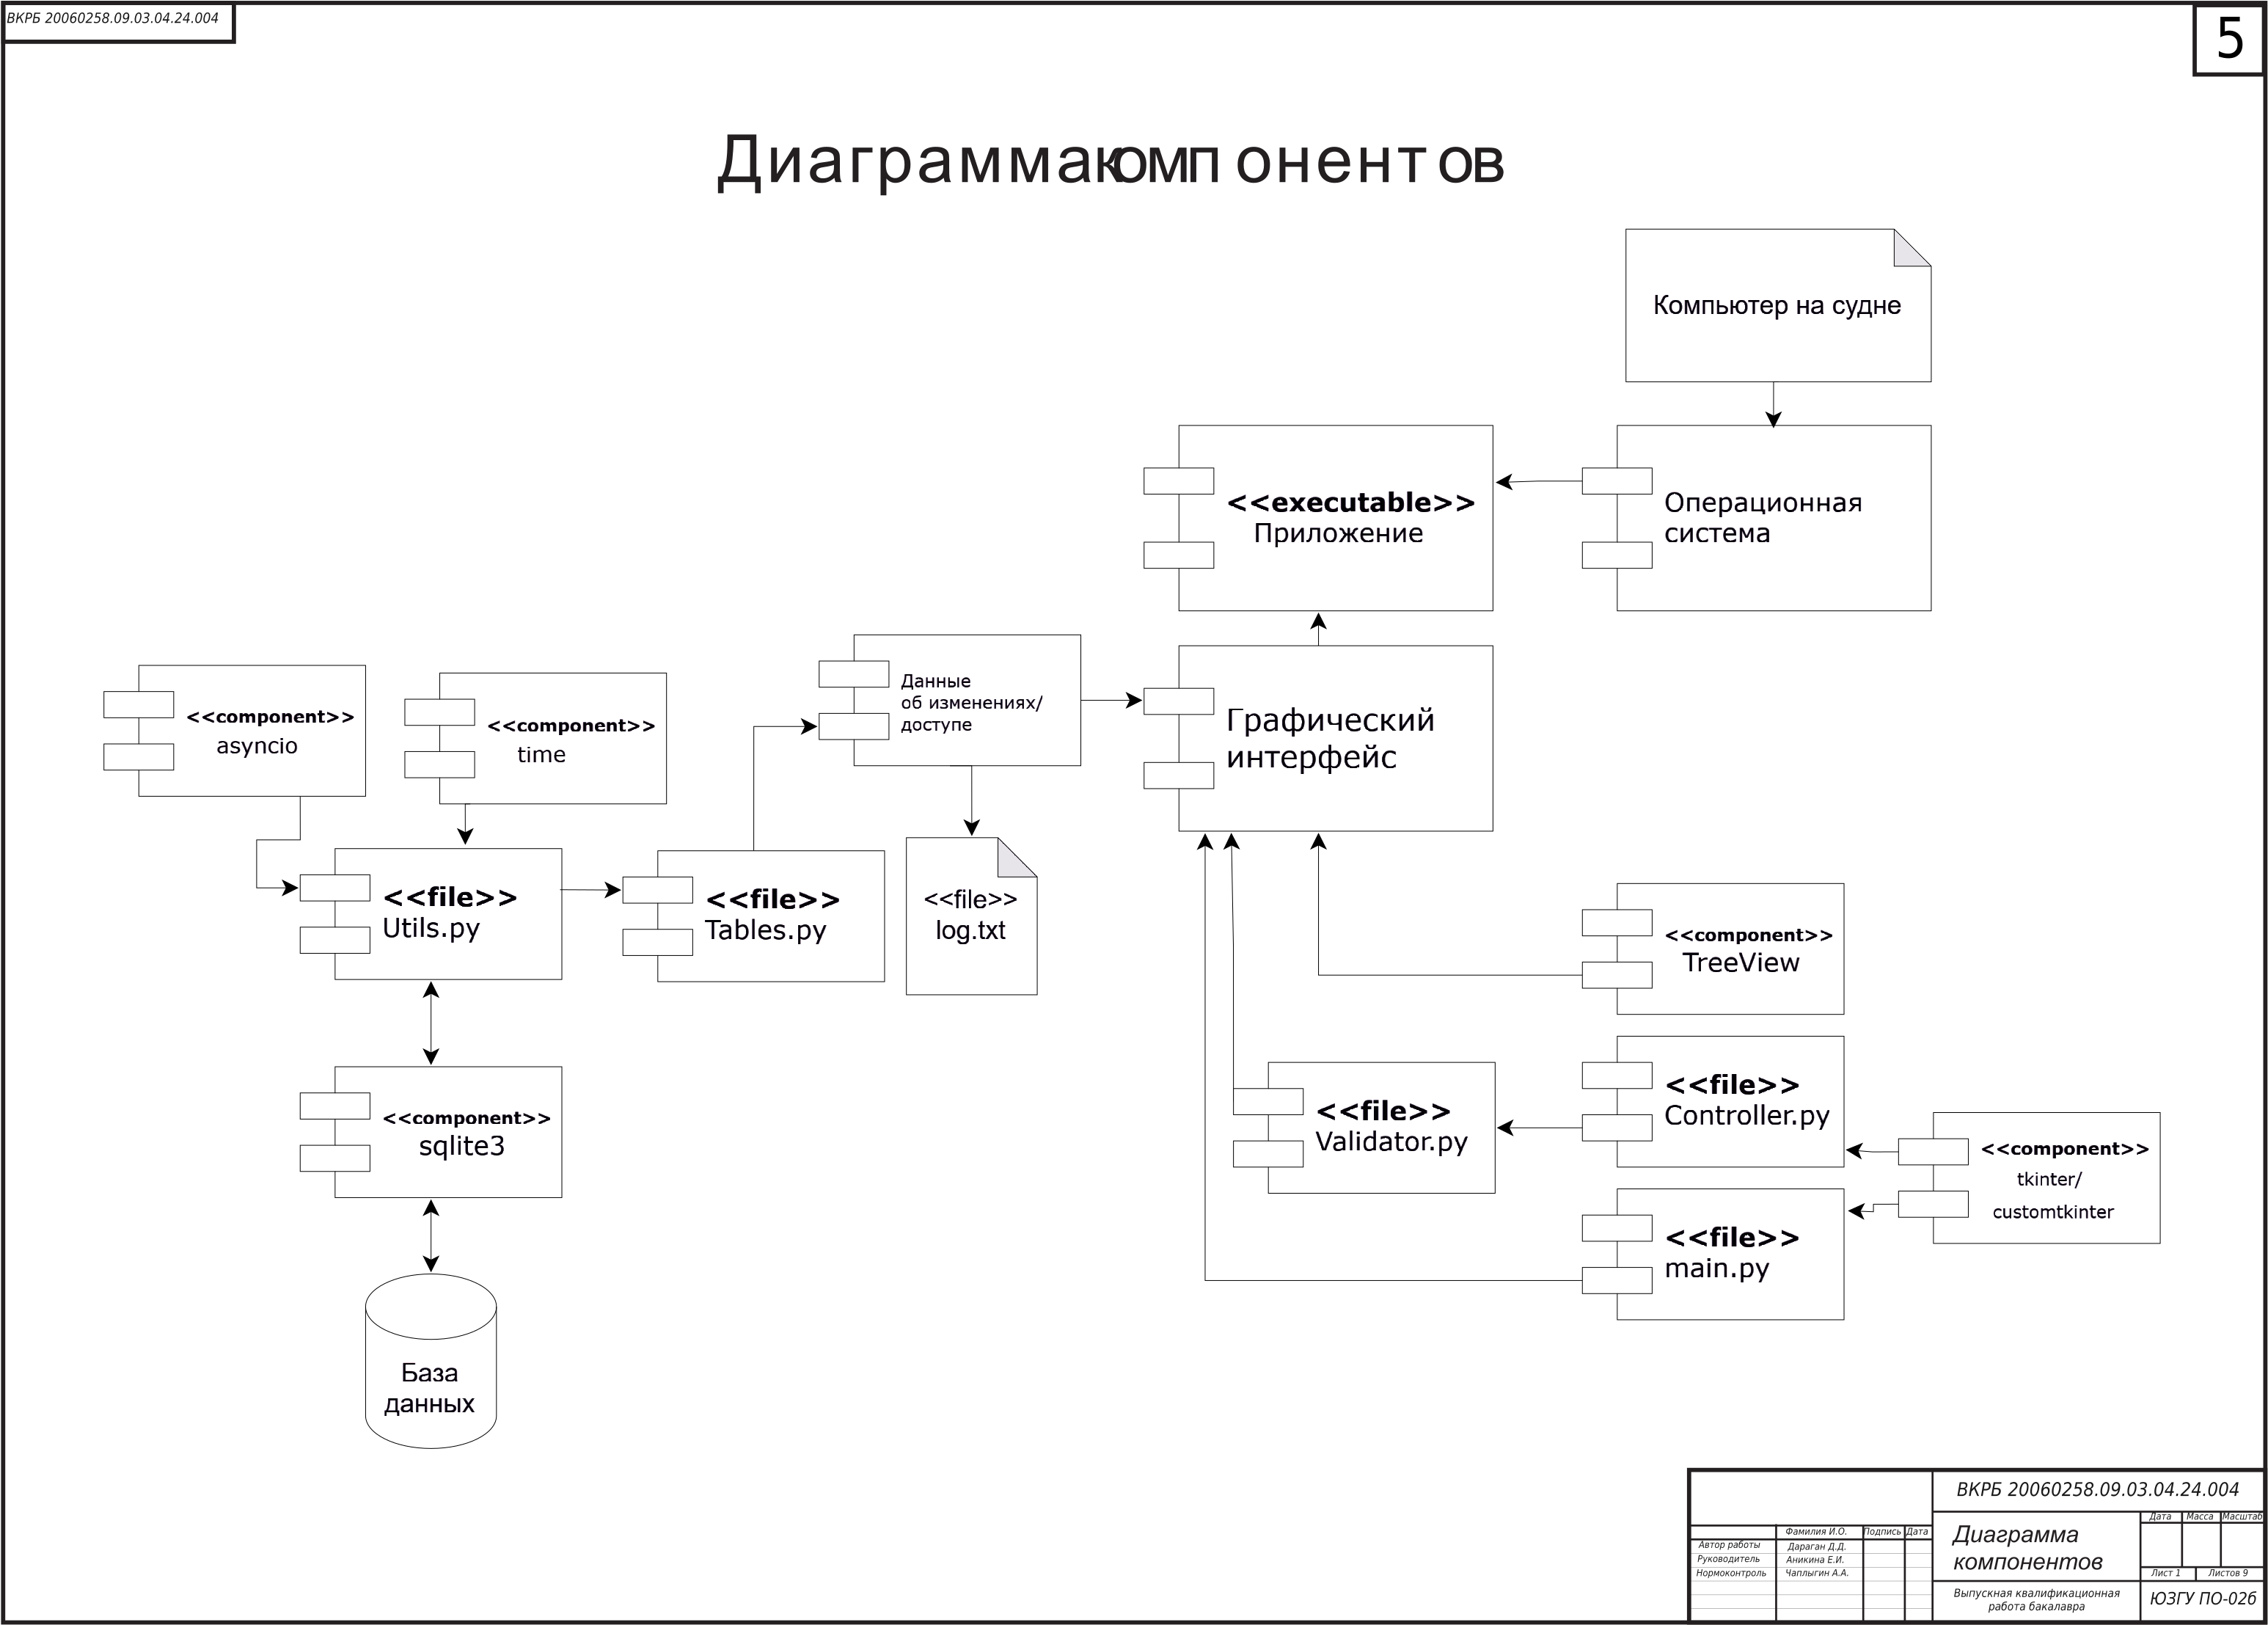
\includegraphics[width=0.82\linewidth]{images/плакат5.png}
	\заголовок{Диаграмма компонентов}
	\label{fig:5}
\end{плакат}

\begin{плакат}
	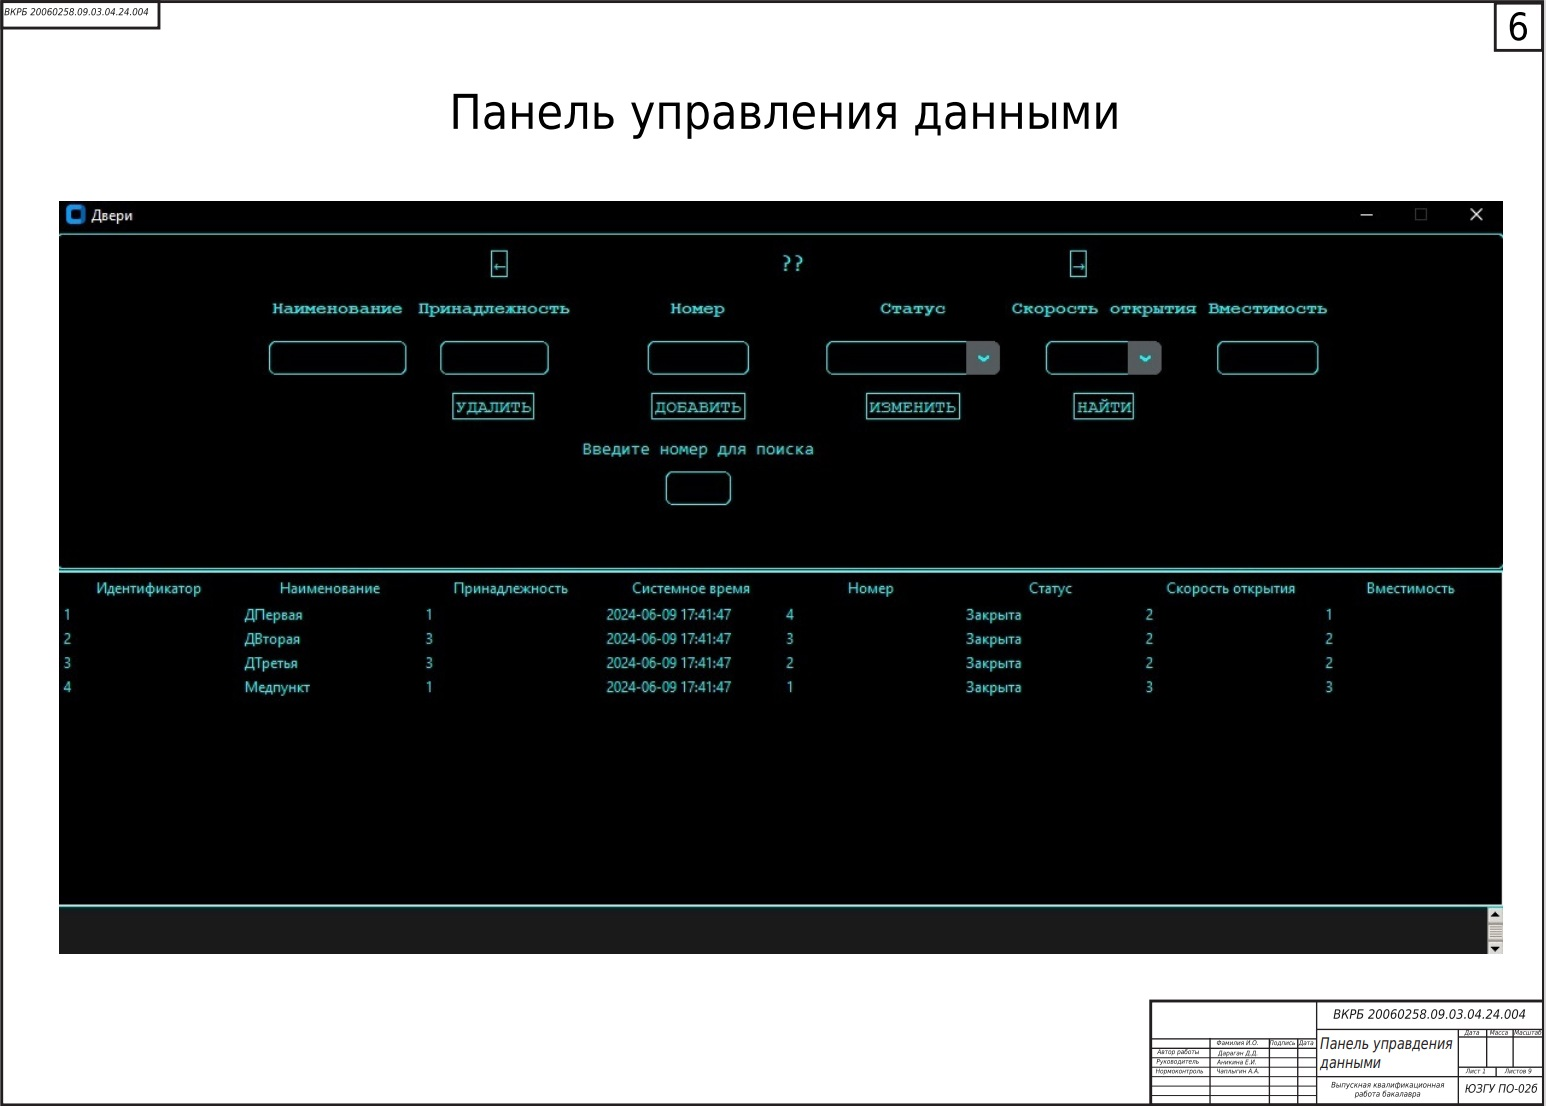
\includegraphics[width=0.82\linewidth]{images/плакат6.png}
	\заголовок{Панель управления данными}
	\label{fig:6}
\end{плакат}

\begin{плакат}
	\centering
	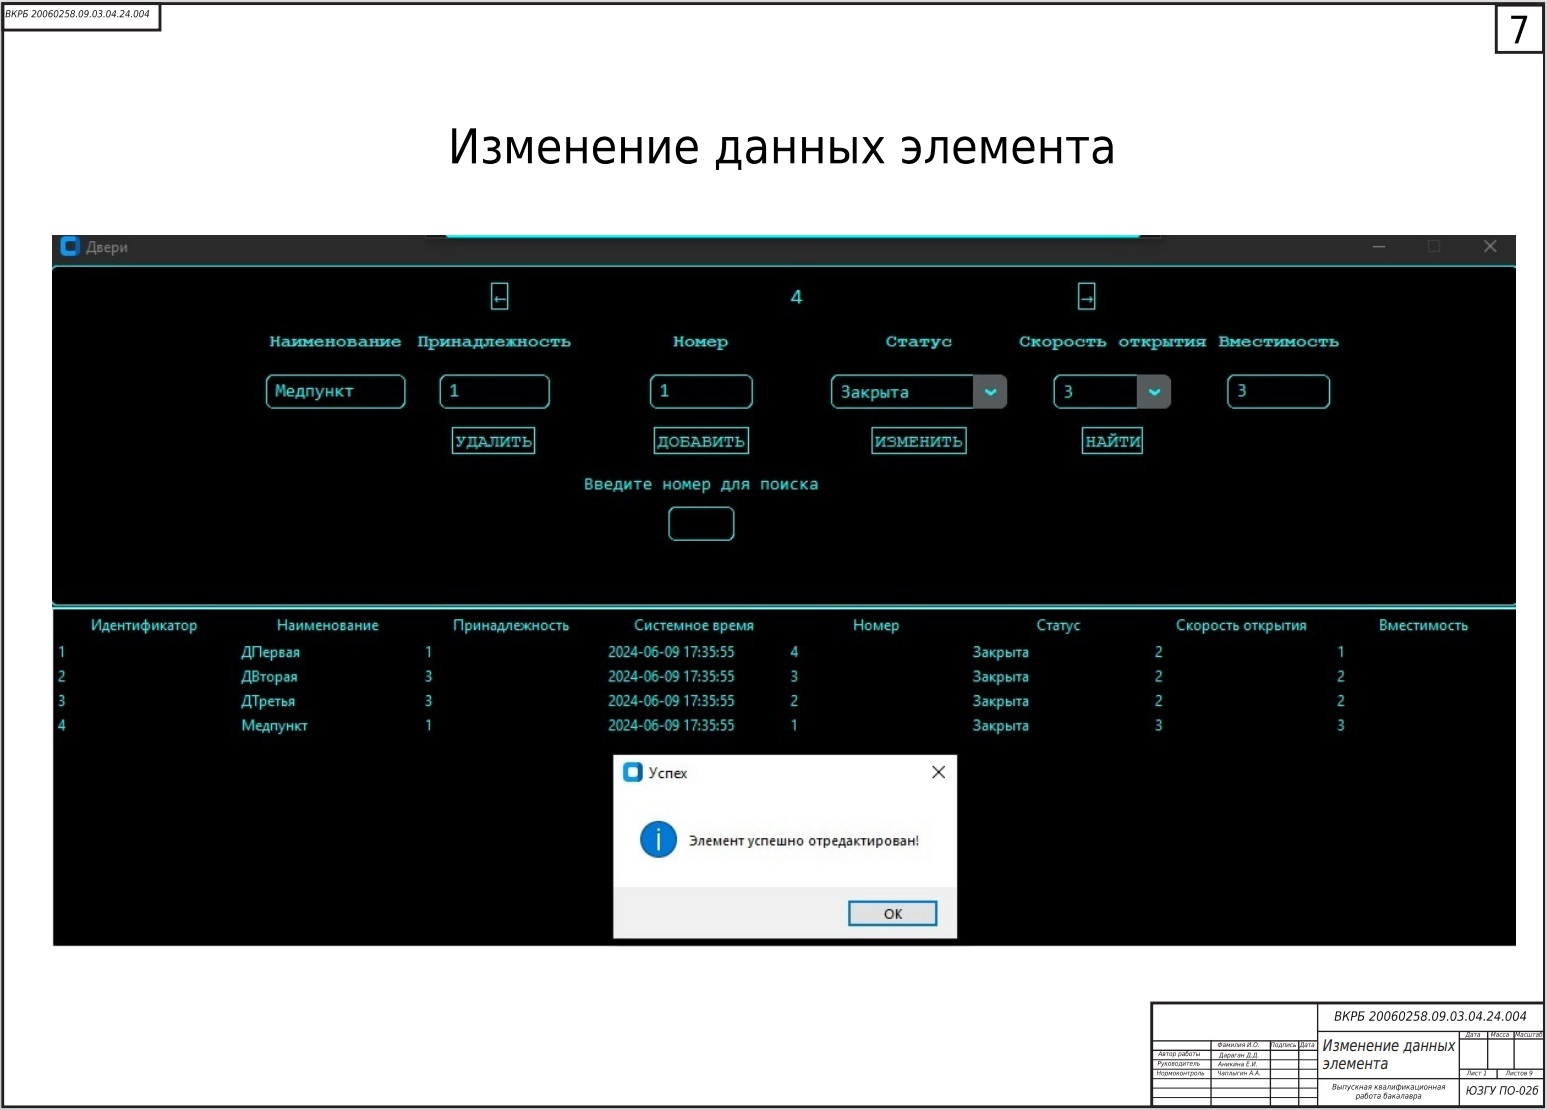
\includegraphics[width=0.82\linewidth]{images/плакат7.png}
	\заголовок{Изменение данных элемента}
	\label{fig:7}
\end{плакат}

\begin{плакат}
	\centering
	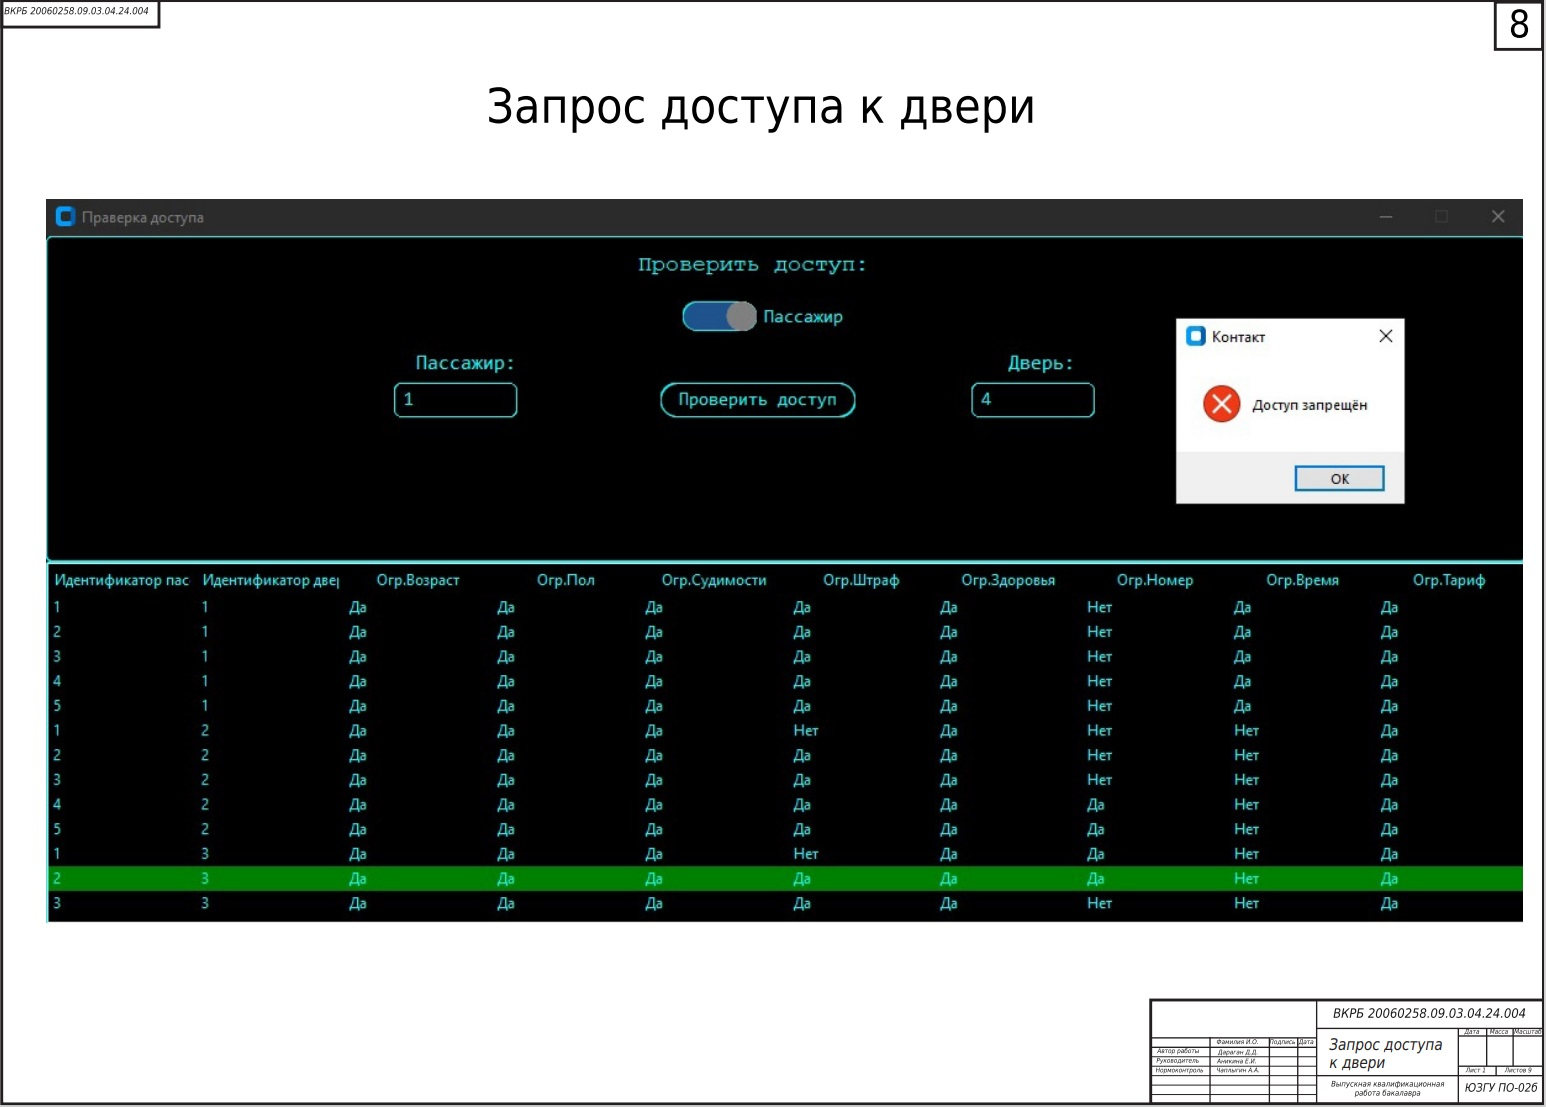
\includegraphics[width=0.82\linewidth]{images/плакат8.png}
	\заголовок{Запрос доступа к двери}
	\label{fig:8}
\end{плакат}

\begin{плакат}
	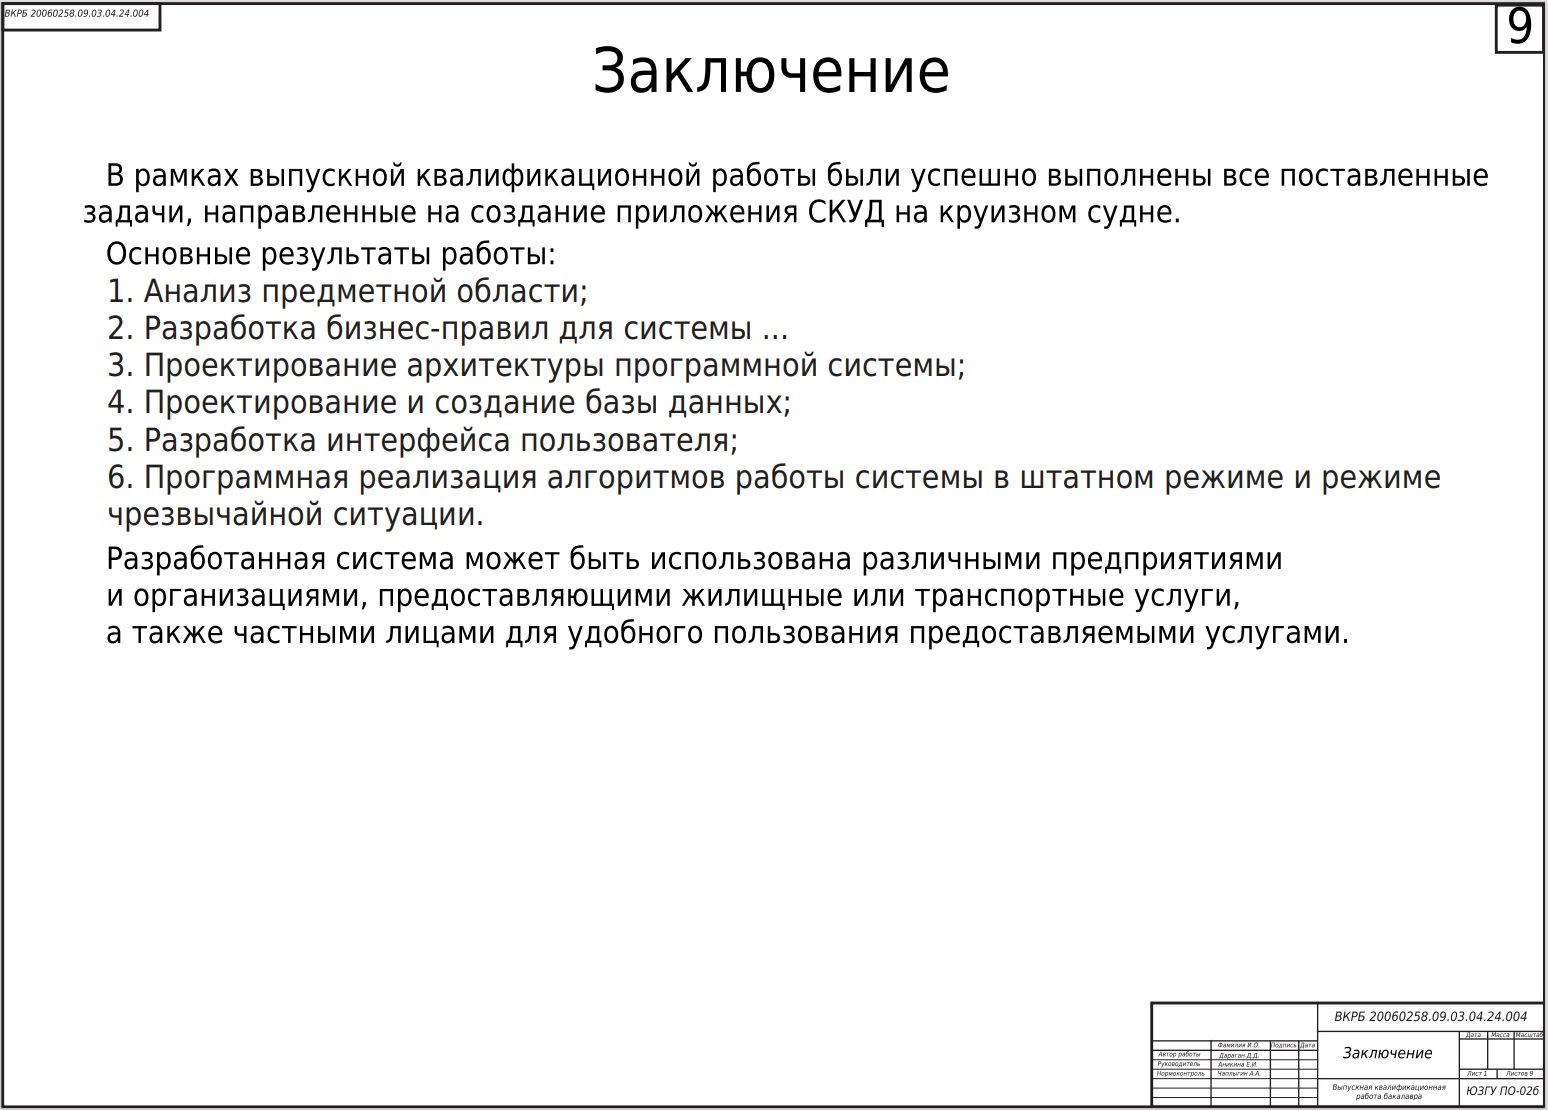
\includegraphics[width=0.82\linewidth]{images/плакат9.png}
	\заголовок{Заключение}
	\label{fig:9}
\end{плакат}

\end{landscape}
